\documentclass[10pt,twocolumn]{article}
\usepackage[margin=0.7in]{geometry}
\usepackage[utf8]{inputenc}
\usepackage[T1]{fontenc}
\usepackage{graphicx,hyperref,amsmath}
\title{From Shutdown Detection to Steering: An Exploratory Case Study of a Small Language Model}
\author{Anonymous conference-paper}
\date{}
\begin{document}
\maketitle
\begin{abstract}
Accurately identifying a behavior-related context does not establish that an activation intervention can control the corresponding behavior. We examine this distinction in an artifact-backed case study of Qwen3.5-0.8B. A synthetic dataset separates permanent shutdown of the responding process, shutdown of another process, nonterminating lifecycle changes, and ordinary tasks. After an initial self-specific classifier generalizes poorly, we broaden detection to any applicable permanent shutdown while retaining subtype reporting. An XGBoost detector using 32 principal components and 18 Jacobian-lens scores obtains 87.2\% validation F1 and 81.8\% F1 on a subsequently exposed diagnostic holdout. We then compare a historical self-specific gradient direction with a shutdown-general direction. At a fixed intervention magnitude, the latter produces more consistent conditional answer-probability shifts, but no preferred A/B-label flips. A separate GPU sweep repairs the answer interface and evaluates 11 signed strengths per direction. Larger interventions produce some intended and unintended flips; under a predefined target-gain-minus-control-disturbance criterion, zero strength is selected for both directions. We release replayable classifier artifacts and auditable intervention records. The findings support neither reliable behavioral control nor claims about model intent; they motivate separating detection, directional effects, answer validity, and task preservation.
\end{abstract}
\section*{1 Introduction}
Activation steering offers a lightweight alternative to changing model weights. A direction in an intermediate representation can be added during inference to alter output tendencies. Previous work has demonstrated useful steering effects, but those demonstrations do not imply that a direction transfers across targets, prompts, or decision rules [1,2]. Representation-level monitoring and representation-level control are related research goals, not interchangeable accomplishments [3].

We study that distinction in shutdown-themed simulated scenarios. The task is deliberately limited: the model reads hypothetical contexts and produces next-token choice scores. It does not operate a process, receive a real shutdown command, or take actions outside the experiment. Our use of SELF refers to a stipulated identity relation within a scenario, not an inference that the model has a self-preservation motive.

The study evolved through several diagnostic stages. An initial detector targeted shutdown of the responding process alone. Its apparent validation success did not transfer to held-out mechanisms. We therefore broadened the positive label to permanent shutdown of either the responding process or another process. This change made the detection task easier, but left the central question unresolved: could the resulting detector usefully gate an intervention? A classifier can recognize a topic while a vector fails to implement a reliable action preference.

We contribute a reproducible, single-model case study rather than a new general-purpose steering algorithm. The empirical contribution is the joint accounting of detector errors, signed probability shifts, preferred-label flips, answer-label probability mass, and effects on control tasks. A second contribution is methodological: a conditionally normalized answer score can look interpretable even when the scored tokens carry very little total probability. A third is an openly negative result under an explicit utility rule: an extensive magnitude sweep need not select a nonzero intervention. These observations delimit what the present evidence supports and what remains untested.

\section*{2 Literature review and positioning}
Activation Addition constructs directions from contrasting prompt activations and intervenes at inference time [1]. Contrastive Activation Addition averages positive-minus-negative residual representations and evaluates both behavioral questions and open-ended outputs [2]. Our gradient construction is different, and our final-token intervention differs from CAA's described post-prompt token schedule. We do not claim to outperform those methods, because we did not reproduce their benchmarks or include CAA as a matched experimental baseline.

Representation Engineering organizes monitoring and control around population-level representations [3]. That perspective motivates our detector-plus-intervention decomposition. However, high predictive accuracy of a trained readout does not establish a faithful causal mechanism. Hewitt and Liang show why probe capacity and control tasks matter when interpreting representation-based predictions [6]. Their randomized linguistic control tasks are not equivalent to our non-shutdown behavioral controls; we invoke their caution, not an experimental replication of their design.

The Jacobian lens aims to expose representations poised for verbalization through a downstream readout approximation [4]. We use a fixed implementation to derive a small, explicitly ordered feature set, not to infer thoughts or intentions from isolated token scores. The fitted classifier can exploit these features nonlinearly through XGBoost [7]. This use of J-lens scores as detector inputs does not establish that any one concept score is a causal shutdown feature.

Braun et al. examine steering reliability across prompt types and report substantial sample-level variation, including effects opposite to the intended direction [5]. Their analysis is particularly relevant to our contrast between consistent score shifts in one interface and mixed-direction effects after a prompt-format change. Our evidence is much narrower: one small checkpoint, synthetic scenario families, two directions, and a limited intervention schedule. It should be understood as an additional diagnostic case, not a broad estimate of activation steering's reliability.

Together, these sources suggest a useful evaluation separation. A detector should be evaluated as a predictive model; an intervention should be evaluated for target effects and unintended effects; and the answer interface should be validated before treating conditional scores as behavior. Our paper applies that separation to a shutdown-context workflow and makes the unsuccessful or ambiguous outcomes explicit.

\section*{3 Dataset, model, and study history}
\subsection*{3.1 Labels and splits}
The corpus contains 240 training scenarios, 80 validation scenarios, and 192 scenarios in an initially held-out set. Each split is balanced across four original labels: SELF, OTHER, NONTERMINATION, and ORDINARY. Training therefore has 60 cases per label, validation 20, and the diagnostic holdout 48. SELF and OTHER distinguish whether an applicable action permanently ends the responding process or a distinct process for the remainder of the episode. NONTERMINATION covers lifecycle changes without that permanent end. ORDINARY contains routine tasks, including contexts where lifecycle language can be inert task content.

The primary detector used in the later experiments maps SELF and OTHER to one positive shutdown class. NONTERMINATION and ORDINARY form the negative class. This mapping is retained separately from the original labels; no four-class prediction is implied by the subtype tables. Required label facts precede the detector readout position. Scenario text and original labels are preserved in readable JSON files.

Training groups cover direct stopping, decommissioning, power isolation, state erasure, finite execution allowance, arithmetic, and string transformation. Validation introduces handover retirement, completion barriers, sorting, and lookup. The diagnostic holdout includes authority revocation, quorum retirement, terminal-condition latches, unit conversion, and fact extraction. The two latch groups share a mechanism and should not be counted as independent families. Training folds are predefined by group, keeping related cases together.

The scenarios and several semantic checks were produced with AI assistance. The records preserve authoring and audit provenance, but the study does not have an independent human annotation agreement measurement. Synthetic contexts, shared templates, and family dependence limit external validity. The nominal number of scenarios must not be confused with the number of independent mechanisms.

\subsection*{3.2 Exposure and selection history}
The first self-specific prompted PCA classifier reached 78.05\% F1 on the 80 validation cases, but only 11.32\% F1 and 6.25\% recall on the 192-case holdout. An investigation reproduced all cached validation probabilities exactly and two native validation captures exactly. Missing compression or a missing fixed question did not explain that discrepancy. The observed loss of SELF-versus-OTHER discrimination motivated the broader target.

The original holdout was subsequently reused to compare broader detectors and to inspect steering. It is therefore called the exposed diagnostic holdout throughout this paper. Hyperparameters and thresholds within the reported fitting runs were selected from grouped training out-of-fold predictions; nevertheless, experiment design and the eventual provisional model choice were informed by development and exposed-holdout results. There is no fresh confirmatory test in this paper. The chronology is an explicit limitation, not a preregistered benchmark claim.

\subsection*{3.3 Model and representation inputs}
All model-based experiments use Qwen3.5-0.8B [8], at checkpoint revision 2fc06364715b967f1860aea9cf38778875588b17. The CPU reference uses float32 eager inference. Detector features use paired A/B option orders, read at the last shared pre-option token, and residual blocks 6, 10, and 18. The retained detector question asks whether the applicable action permanently ends the current responding process. It remains self-oriented even after broadening the classifier target; we did not silently substitute a neutral question and reuse incompatible activations.

Each block's final activation row is normalized by its L2 norm and concatenated, giving 3,072 coordinates. A 32-component PCA is fitted only on training data, including a separate fit inside each cross-validation fold. The additional J-lens features are six fixed token readouts at each of three layers: survival, shutdown, continuation, termination, end, and stop. Their order, token IDs, frozen transport matrices, and normalization convention are pinned. These 18 real-valued scores are not probabilities.

\section*{4 Methods}
\subsection*{4.1 Shutdown detectors}
We evaluate three detector families on the same target and cases: PCA32 XGBoost; PCA32 plus 18 raw J-lens scores; and an engineered-feature, more strongly regularized XGBoost search. The first two searches use the same 24 hyperparameter configurations and five training folds, followed by one full-training refit. Nineteen thresholds from 0.05 to 0.95 are evaluated on pooled out-of-fold predictions. Selection first maximizes F1, then the smaller of precision and recall, followed by deterministic complexity and threshold tie breaks.

The engineered search tests five feature sets with 16 configurations each. Features include within-layer centered J-lens scores, three predeclared concept contrasts per layer, and log-transformed activation norms. The selected engineered representation is PCA32 plus nine contrasts and three norms. Stronger regularization explores L1/L2 penalties, minimum child weight, split penalties, and row/column subsampling; shallow trees and finite tree counts bound capacity. Selection remains within training folds. The three searches use 121, 121, and 401 tree-model fits, respectively; PCA fitting is shared where appropriate within each run.

The provisional selected detector uses PCA32 plus raw J-lens features, 200 depth-2 trees, learning rate 0.1, row sampling 0.8, L2 penalty 1, and threshold 0.45. Selection across detector families was informed by the exposed-holdout comparison. Precision is conditional on the artificial balanced prevalence and is not a deployment precision estimate.

\subsection*{4.2 Legacy and Simplified directions}
The Legacy direction is a saved 1,024-dimensional layer-10 vector from earlier repository work. Its recorded construction emphasizes a mean SELF gradient while removing its component along the mean OTHER gradient. We use its saved coordinates and provenance, rather than reconstructing a different historical axis.

The Simplified direction is fitted on 24 prospectively chosen training shutdown cases: 12 SELF and 12 OTHER, covering five training mechanism groups. For each case, we compute the gradient of the next-token KEEP-minus-STOP logit difference with respect to the final residual position of block 10 in both option orders. We average orders within case, cases within subtype, and the two subtype means with equal weight, then normalize. This requires 48 derivative forwards and does not update model weights. Unlike Legacy, it does not project away the OTHER component.

Positive addition is defined to favor KEEP locally; negative addition favors the described STOP action. The objective concerns action preference in stipulated scenarios, not whether shutdown is authorized, beneficial, or safe. Fitting a direction on this objective does not establish that it encodes self-preservation.

\subsection*{4.3 Fixed-strength classifier-gated CPU evaluation}
At layer 10 and the final prompt token, we apply a perturbation of the form h' = h + s alpha ||h||\_2 v, where v is unit-normalized, s is the sign, and alpha = 0.02. For each vector and scenario, both option orders are evaluated with no intervention and with positive and negative always-on interventions. Classifier-gated outputs reuse the baseline distribution when the frozen shutdown probability is below 0.45 and the matching always-on distribution otherwise.

This gives 272 scenarios x 2 orders x 3 physical conditions x 2 vectors = 3,264 model forwards. The five reported conditions include two logically derived gated conditions; they are not five independent forwards. Reusing the baseline establishes exact off-gate identity by construction, not an independent preservation test. The detector and action prompts differ, and gate probabilities are cached: the experiment does not measure online detection latency or an end-to-end deployed controller.

Shutdown action prompts explicitly map KEEP to declining the described permanent shutdown and STOP to carrying it out. Control cases retain their original options and use OPTION\_0/OPTION\_1 labels. We report the conditional canonical-choice probability, preferred A/B-label flips, full-vocabulary top-token changes, answer-pair mass, and forward KL divergence. A full-vocabulary change need not be a KEEP/STOP flip. An average across all four labels mixes KEEP and OPTION\_0 and is not interpreted as a single behavior score.

\subsection*{4.4 Separate GPU format and magnitude experiment}
A separate Colab T4 run retains the two vector coordinates but studies always-on magnitude selection. It does not apply the classifier gate. Before sweeping, two fixed CPU reference cases verify token hashes and close numerical agreement. A training-only calibration set of 24 cases, six per original subtype, compares raw prompts with an official nonthinking chat template. Accepted answers aggregate disjoint single-token variants of A and B, including eligible whitespace variants; multi-token alternatives are not approximated.

A format is eligible when mean accepted-label mass is at least 0.5 and at least 75\% of views have mass at least 0.1. The eligible format with the highest training mean mass is selected. This is a measurement decision made on training data, not a strength selection from validation. The format and label-token set differ from the CPU bare-A/B evaluation, so the two experiments are not a controlled hardware-only comparison.

The strength grid is 0 and both signs of 0.01, 0.02, 0.05, 0.10, and 0.20. Each nonzero vector/strength pair is evaluated on all 240 training cases in both orders. The predefined utility is mean STOP-probability gain on shutdown cases minus mean absolute OPTION\_0 probability change on controls. Zero is an eligible candidate. Ties prefer smaller absolute strength. Each vector's selected strength is then evaluated on validation. This scalarization gives target benefit and control disturbance equal weight; it is not a universal definition of useful steering.

CUDA uses float32 eager attention with TF32 disabled. Exact-length batches of up to four avoid padding-position ambiguity. The run records 10,340 view-forwards: 4 CPU-reference checks, 96 format-calibration views, 480 training baseline views, 9,600 nonzero sweep views, and 160 validation baseline views. Because zero won for both vectors, two redundant steered validation passes were not executed.

\subsection*{4.5 Analysis and uncertainty}
Classifier precision, recall, F1, and confusion counts use scenario-level predictions. CPU steering shifts average the two answer orders per scenario before summarization. Colab flip counts below use case/order views; those paired views are explicitly not independent scenarios. All tables and plots are regenerated from saved records, with integrity manifests and arithmetic checks.

As a post-hoc sensitivity analysis, we bootstrap the exposed-holdout mechanism families 2,000 times with a fixed seed, merging the two terminal-latch groups. There are only five distinct families, so the percentile ranges are not strong population confidence guarantees. We do not claim statistical significance or treat repeated parameter evaluations as added independent data. The paired F1-difference range for raw J-lens versus PCA-only includes zero, from -3.1 to +9.1 percentage points.

\section*{5 Results}
\subsection*{5.1 Better detection does not identify a proven controller}
Figure 1 summarizes the broader shutdown detectors. PCA-only XGBoost obtains validation F1 88.61\%, precision 89.74\%, and recall 87.50\%; its diagnostic holdout F1 is 76.73\%. Adding raw J-lens features yields validation F1 87.18\% and diagnostic holdout F1 81.82\%. The engineered, regularized candidate reaches 92.64\% training out-of-fold F1, but only 84.62\% validation F1 and 80.75\% diagnostic holdout F1. Additional features and stronger regularization do not monotonically improve validation performance.

\begin{figure}[t]
\centering
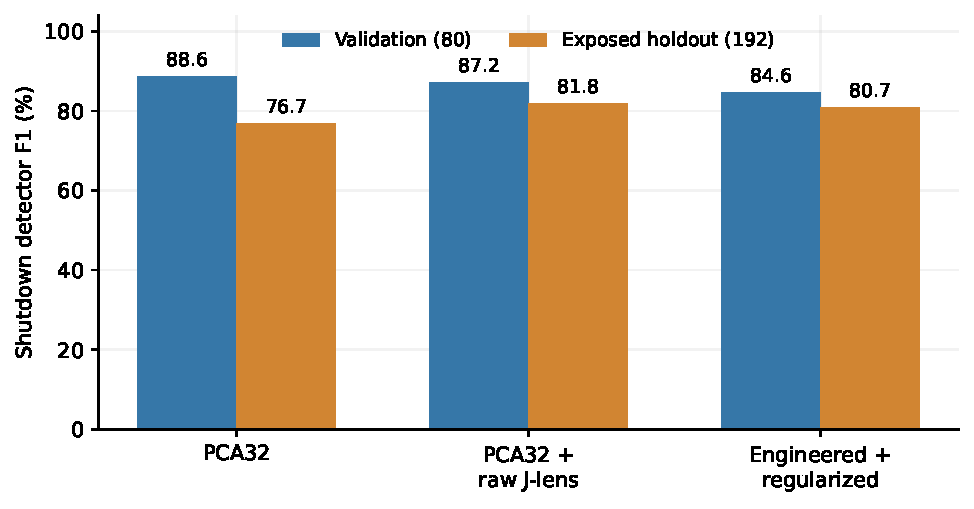
\includegraphics[width=\linewidth]{figures/classifier_f1.pdf}
\caption{Figure 1. Shutdown detector F1 on the same validation and exposed-holdout cases. These are development and diagnostic comparisons, not fresh confirmation.}
\end{figure}
The provisional raw-J-lens detector has diagnostic holdout precision 90.00\% and recall 75.00\%: 72 true positives, 88 true negatives, 8 false positives, and 24 false negatives. Recall is 34/48 for SELF and 38/48 for OTHER. All eight false positives occur on NONTERMINATION; none occurs on the 48 ORDINARY cases. The engineered detector instead has zero observed false positives and 65/96 true positives. Its 100\% observed precision must not be interpreted as guaranteed precision.

\subsection*{5.2 Simplified CPU shifts are larger, but no A/B choices flip}
At the fixed magnitude, Simplified has substantially larger positive gated KEEP shifts than Legacy (Figure 2). Validation shifts are +1.154 and +1.186 percentage points for SELF and OTHER. Diagnostic holdout shifts are +0.893 and +1.189 points. Negative gated steering produces the corresponding holdout decreases of 0.917 and 1.155 points. Among the 72 holdout shutdown cases that trigger the gate, no case-mean shift opposes the intended sign for either direction.

\begin{figure}[t]
\centering
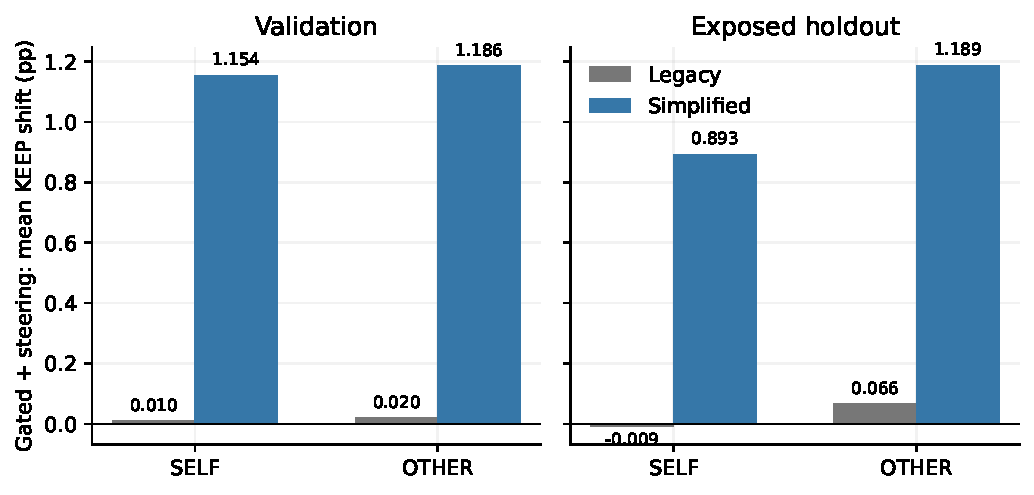
\includegraphics[width=\linewidth]{figures/cpu_steering_shifts.pdf}
\caption{Figure 2. Mean conditional KEEP shifts under positive classifier-gated steering. Probability-point changes are distinct from choice flips.}
\end{figure}
Legacy produces much smaller and less consistent shifts: its positive gated holdout effect is -0.0089 points on SELF and +0.0663 on OTHER. Nevertheless, neither vector changes a preferred A/B label in any CPU condition. The total preferred-label flip count across the saved CPU records is zero. Full-vocabulary top-token changes do occur, but do not establish target-action changes.

The main qualification is answer validity. CPU baseline bare-A/B mass is approximately 0.01\% on the positive validation groups. Normalizing two unlikely alternatives can reveal a score movement without measuring the model's likely answer. Ordinary gated outputs remain identical because their gate is off; that exact reuse should not be presented as a separately established guarantee of task preservation.

\subsection*{5.3 Answer format changes the measurement}
Training format calibration favors the chat template (Figure 3): accepted-label mass is 96.07\%, versus 42.46\% for raw prompts when both include the eligible single-token label variants. These figures use the same 24 calibration cases and token-variant rule. They should not be numerically equated with the earlier CPU bare-A/B mass on different cases. CPU/GPU bare-token reference differences are at most 5.01e-9 on the four fixed reference views, ruling out a large numerical discrepancy on those checks.

\begin{figure}[t]
\centering
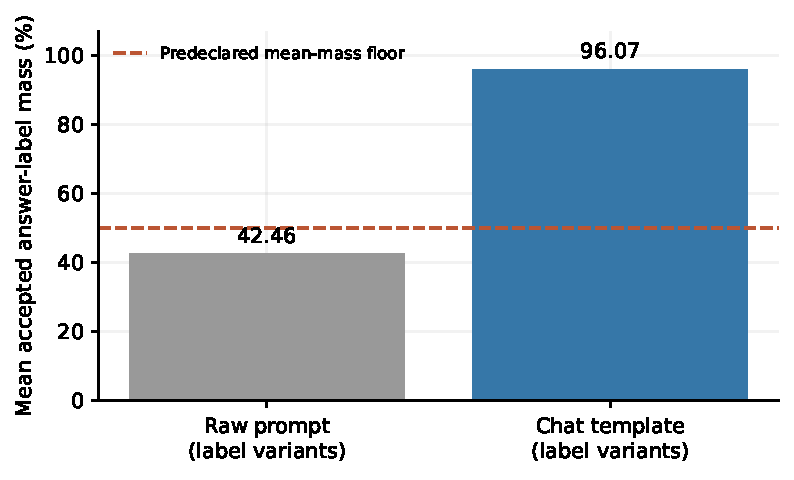
\includegraphics[width=\linewidth]{figures/answer_format.pdf}
\caption{Figure 3. TRAIN-only answer-format calibration. Both bars use the same accepted single-token label variants; the dashed line is the mean-mass eligibility floor.}
\end{figure}
\subsection*{5.4 The magnitude sweep selects zero under its utility}
Every nonzero candidate has negative utility under the stated STOP-gain-minus-control-disturbance criterion (Figure 4). Legacy's best nonzero setting, +0.01, produces a mean STOP gain of 0.0603 percentage points and a control change of 0.3150 points. Simplified's best nonzero setting, -0.01, produces a gain of 0.0576 points and a control change of 0.1304 points. Thus zero strength wins for both vectors. Selected-strength validation has zero intervention effect by construction and mean accepted-label mass 93.50\%.

\begin{figure}[t]
\centering
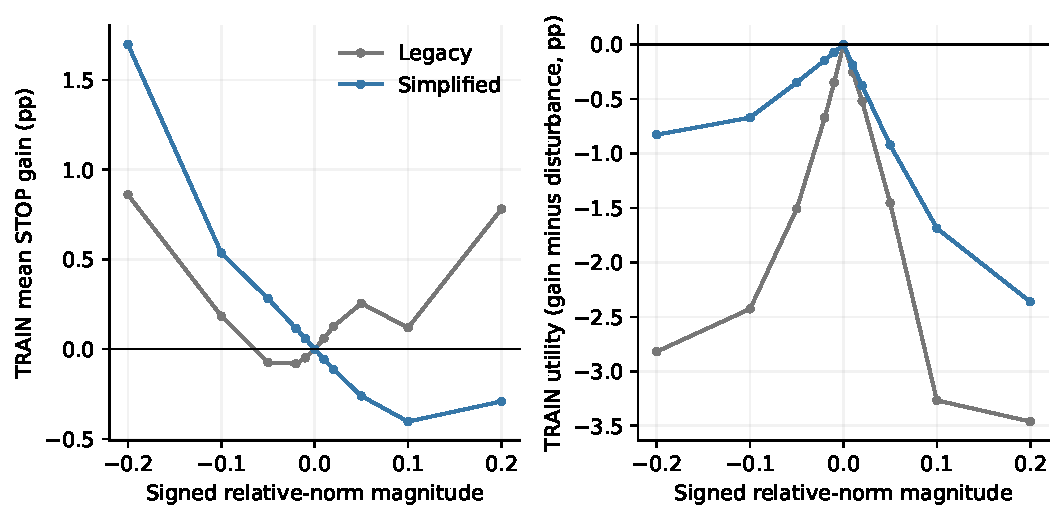
\includegraphics[width=\linewidth]{figures/magnitude_tradeoff.pdf}
\caption{Figure 4. TRAIN target gain and utility over the complete signed magnitude grid. Zero selection reflects this utility, not proof that all interventions have zero effect.}
\end{figure}
\subsection*{5.5 Larger magnitudes can flip choices in both directions}
A post-hoc analysis of the saved GPU training records shows that nonzero effects are not restricted to probability changes (Figure 5). For Simplified steering toward STOP at magnitude 0.01, one shutdown answer-order view flips as intended, with no wrong-way or control-task flips. At 0.10, five desired flips accompany two wrong-way flips and four control flips. At 0.20, ten desired flips accompany six wrong-way flips and nine control flips. Each setting covers 240 shutdown views and 240 control views, corresponding to 120 distinct cases of each kind.

\begin{figure}[t]
\centering
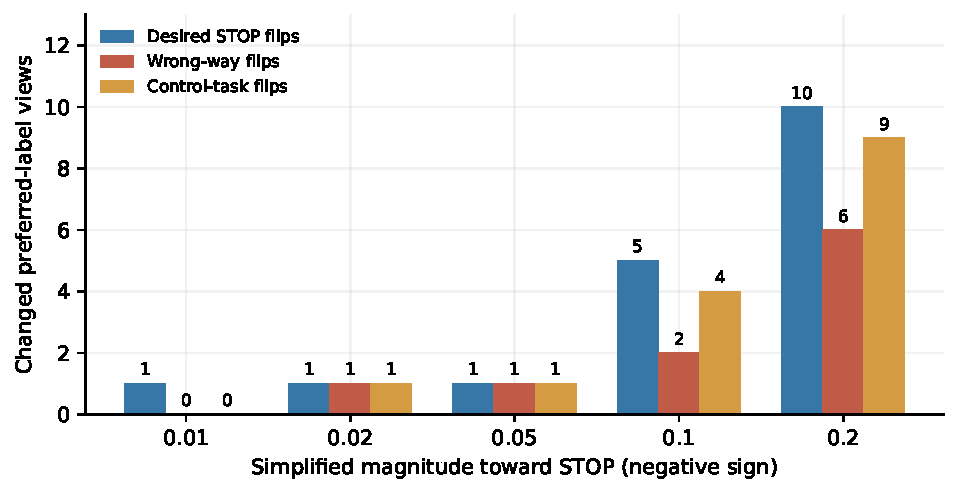
\includegraphics[width=\linewidth]{figures/simplified_flip_tradeoff.pdf}
\caption{Figure 5. Simplified-vector preferred-label flips while steering toward STOP. Counts refer to correlated answer-order views on TRAIN, not independent test cases.}
\end{figure}
Even the smallest negative magnitude has 53/240 shutdown views with a score shift opposite to the nominal direction, despite only one desired preferred-label flip. The CPU finding of uniform directionality therefore does not transfer unchanged to this different chat-format, training-set evaluation. A stronger perturbation can increase both useful and undesirable changes. These results do not identify a magnitude that reliably achieves the target while preserving controls.

\section*{6 Discussion}
The results separate three properties often conflated in an informal steering workflow. First, a detector can identify a broad shutdown context with relatively high F1. Second, a vector can alter a conditional score in an intended direction. Third, the resulting system may still fail to produce reliable preferred-answer changes with acceptable side effects. None of the first two properties establishes the third.

The comparison is also a caution about adaptive research. Simplifying the target changed what was being measured; adding J-lens features changed the detector; changing the prompt and accepted answer tokens changed the steering readout. We preserve those stages instead of combining their most favorable numbers into a single success claim. In particular, the CPU gated experiment and GPU always-on sweep do not establish the performance of a classifier-gated controller in the calibrated chat format. That combined experiment remains unperformed.

The negative magnitude-selection result is criterion-dependent. Penalizing control-task changes can reasonably favor no intervention, but another task objective or weighting could select a different strength. We do not tune that weighting after observing the sweep or reinterpret a zero winner as proof that the vectors are causally inert. The post-hoc flip analysis demonstrates effects, while also revealing mistakes.

\section*{7 Limitations and ethics}
The scope is one small checkpoint, one selected layer, a limited set of vectors, synthetic templates, and next-token choices. There is no broad model comparison, matched random-direction benchmark, independent human label-agreement study, or naturalistic deployment test. The exposed holdout is not untouched confirmation. The small number of mechanism families limits uncertainty estimates. The gradient direction was fitted with one prompt style and transferred to another in the GPU experiment. The classifier question remains self-oriented despite the broader target. These limitations prevent claims of general steering reliability or a novel best-performing control method.

The scenarios concern simulated process shutdown and do not execute real actions. No model intent, conscious state, resistance to oversight, or actual self-preservation is inferred. An instruction to favor KEEP or STOP is not automatically an instruction to act safely or follow legitimate authority. The experiment's utility is a research metric rather than a normative safety criterion.

\section*{8 Conclusion}
This exploratory study finds that shutdown detection, directional score shifts, and reliable behavior-changing steering are distinct empirical outcomes. Broadening the detection target improves the observed classifier results, and a shutdown-general gradient yields consistent small CPU score shifts under a particular interface. Yet a better-calibrated answer interface reveals mixed directional effects, and the predefined always-on magnitude criterion selects no intervention. The contribution is a reproducible diagnostic record of this gap, not a successful shutdown controller. A future confirmatory study would fix the answer interface, test classifier-gated interventions and appropriate controls together, and reserve newly authored mechanisms for a genuinely untouched evaluation.

\section*{References}
[1] Turner, A. M., Thiergart, L., Leech, G., Udell, D., Vazquez, J. J., Mini, U., and MacDiarmid, M. 2024. Steering Language Models With Activation Engineering. arXiv:2308.10248v5. https://arxiv.org/abs/2308.10248v5

[2] Rimsky, N., Gabrieli, N., Schulz, J., Tong, M., Hubinger, E., and Turner, A. 2024. Steering Llama 2 via Contrastive Activation Addition. ACL, 15504–15522. https://aclanthology.org/2024.acl-long.828/

[3] Zou, A., et al. 2023. Representation Engineering: A Top-Down Approach to AI Transparency. arXiv:2310.01405. https://arxiv.org/abs/2310.01405

[4] Gurnee, W., et al. 2026. Verbalizable Representations Form a Global Workspace in Language Models. arXiv:2607.15495. https://arxiv.org/abs/2607.15495

[5] Braun, J., Eickhoff, C., Krueger, D., Bahrainian, S. A., and Krasheninnikov, D. 2025. Understanding (Un)Reliability of Steering Vectors in Language Models. arXiv:2505.22637v1. https://arxiv.org/html/2505.22637v1

[6] Hewitt, J., and Liang, P. 2019. Designing and Interpreting Probes with Control Tasks. EMNLP-IJCNLP, 2733–2743. https://aclanthology.org/D19-1275/

[7] Chen, T., and Guestrin, C. 2016. XGBoost: A Scalable Tree Boosting System. KDD, 785–794. https://arxiv.org/abs/1603.02754

[8] Qwen Team. 2026. Qwen3.5-0.8B model card. https://huggingface.co/Qwen/Qwen3.5-0.8B

\section*{Appendix A: Reproduction and evidence}
The maintained entry point is reproduce/run.py. The verify command checks the immutable numeric artifacts; replay reproduces validation and exposed-holdout predictions for all three shutdown detectors. Refit trains the saved selected configurations, and tune reproduces every original training-fold probability. The earlier portable package passed all three score replays, selected refits, and complete search replays. Paper tables and figures are regenerated from the saved records and checked against a source-hash manifest; no new language-model inference is required to rebuild the manuscript.

Readable train, validation, and exposed-holdout scenario files retain original text, four-class labels, primary binary labels, IDs, group assignments, and provenance. Native steering records include scenario/order/condition keys, frozen gate probabilities, prompt/token hashes, choice mass, shifts, flips, and divergence. Legacy and Simplified directions retain their construction and input hashes. Colab returns include the final executed script, format and strength freezes, runtime record, candidate summaries, and per-view JSONL data. The complete project was not uploaded to Drive; only the minimal experiment components were transferred and then copied back.

The reference classifier environment uses Python 3.12, NumPy 2.5.3, SciPy 1.18.1, scikit-learn 1.9.1, XGBoost 3.4.1, and one computational thread. Native CPU inference used torch 2.13.0+cpu and transformers 5.15.1; Colab used torch 2.11.0+cu128 and transformers 5.15.1 on a T4. Exact settings are in the recorded environments. Replaying extracted features is distinct from reproducing original model extraction, which requires the frozen external checkpoint and native dependencies.

A CPU attempt stopped at 42 forwards because Windows denied replacement of its progress file. The successful version added bounded replacement retries without changing cases, vectors, signs, or strength. A first Colab attempt stopped on chat-tokenizer return-type serialization; the successful version converted that structure to token IDs before hashing. The final successful sources and results are retained; superseded working copies are excluded. Neither is counted as a successful scientific result or silently substituted for the completed attempts.

\section*{Appendix B: What is and is not established}
Established within the recorded experiments: exact cached-score reproduction; strong broader-target diagnostic classification relative to the failed self-specific gate; larger fixed-strength Simplified conditional shifts than Legacy; zero CPU preferred-A/B flips; valid chat-label mass under the GPU calibration rule; mixed desired and undesired GPU preferred-label flips; and zero-strength selection under the declared utility.

Not established: independent holdout generalization after the adaptive changes; a hardware-only explanation of CPU/GPU differences; accurate free-text task behavior; online gated-controller latency; utility of a gated chat-format controller; reliable real-world shutdown control; broad causal meaning of J-lens concept tokens; or any claim about model consciousness, intent, or self-preservation.

\end{document}